\documentclass{article}
\usepackage[utf8]{inputenc}
\usepackage[margin=1in]{geometry}
\usepackage{soul,color}
\usepackage{amsfonts, amsmath}
\usepackage{bbm}
\usepackage{enumitem}
\usepackage{amssymb}
\usepackage{pict2e,graphicx}
\usepackage[nobreak=true]{mdframed}
\usepackage{listings,xcolor}
\usepackage{subfigure}
\lstset{numbers=left,numberstyle=\tiny,keywordstyle=\color{blue},commentstyle=\color[cmyk]{1,0,1,0},frame=single,escapeinside=``,
breaklines,extendedchars=false,xleftmargin=2em,
xrightmargin=2em,aboveskip=1em,tabsize=4,showspaces=false}

\title{Data Simulation}
\author{\vspace{-6ex} Luhuan Wu, Xiaohui Li}
 \date{6-19-2017}
%\date{\vspace{-6ex}}

\begin{document}
\maketitle
\begin{enumerate}

\item Degree sequence generation\\
We generate $W^-$ by 
$$U \sim \text{Uniform}(0, 1), W^{-1}=F^{-1}(U)=c(1-U)^{-\frac{1}{\beta}}$$
And then get generate $W^+$ by
$$W^= = a(W^-)^d$$
And then independently generate $(D^+, D^-) = (Poisson(W^+), Poisson(W^-))$.

\item Tail distribution test\\
We set $c = 5, \beta = 2$, and W has the distribution 
$$P(W> x) = (\frac{x}{c})^{-\beta}, \qquad x >c$$
And $D = Poisson(W)$. \\
We generate independent samples of W and D of sample size 2000 and obtain the log-log plot of tail distribution below:\\
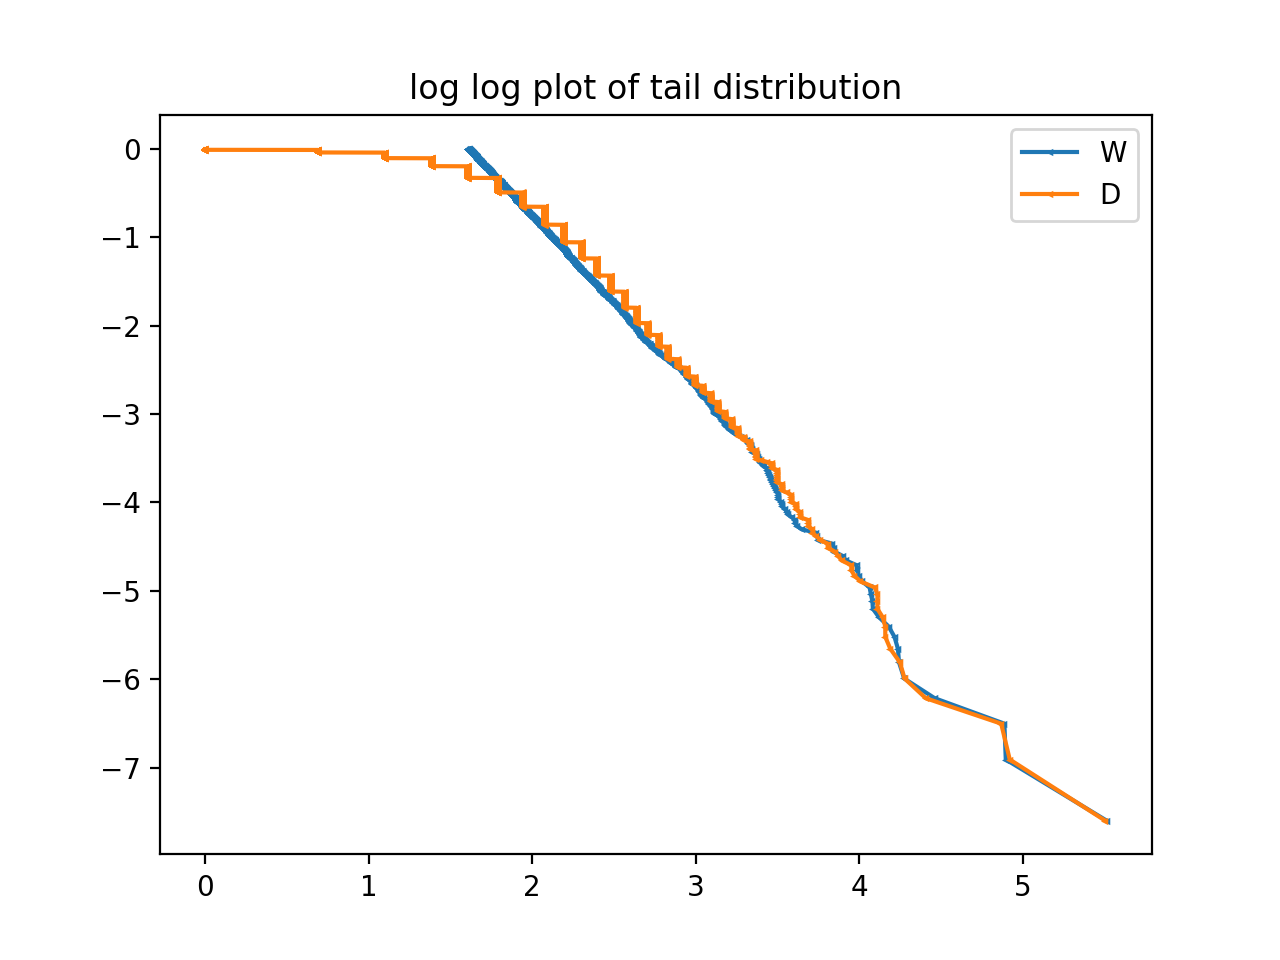
\includegraphics[scale=0.8]{loglog_tail_dist.png}
\\
We can see that the two tails almost coincide and are straight lines.
\item Tail distribution of page rank, betweenness centraliy and in/out degree sequence.\\
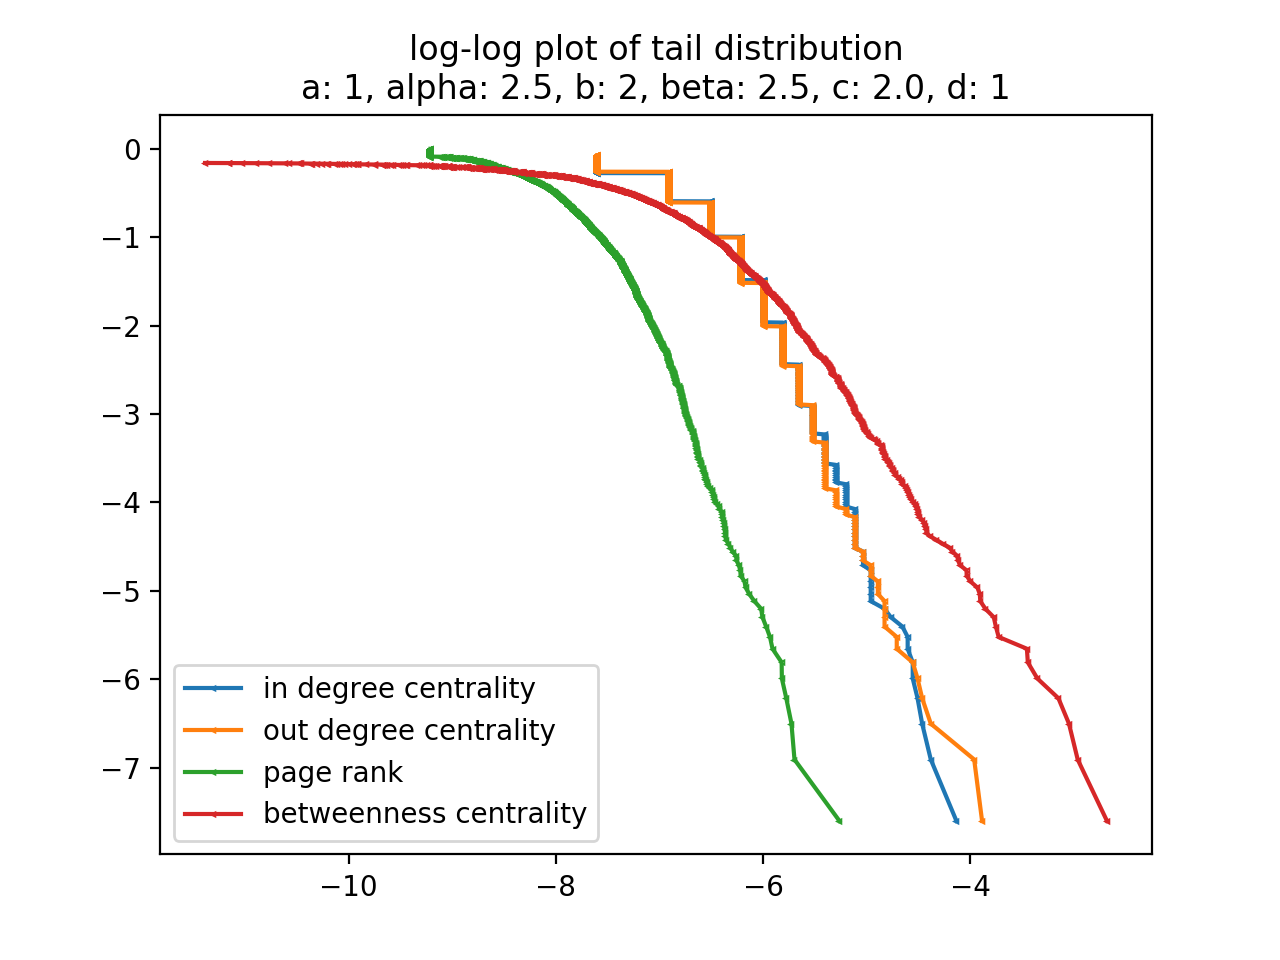
\includegraphics[scale=0.8]{page_rank_degree_centrality.png}
\\
The in (out) degree centrality is (out) degree sequence didivded by max in (out) degree.\\
We can clearly see that the page rank plot is parallel to degree centrality plot.\\

Below are calculations:
\item
This is the basic set-up:
$$P(D^+ = d^+, D^- = d^-) = P(Poisson(W^+) = d^+, Poisson(W^-)=d^-)$$
where $(W^+,W^-)$  are jointly regularly varying.
$$P(W^+ > x) = (\frac{x}{b})^{-\alpha},\qquad x >b$$
$$P(W^- > x) = (\frac{x}{c})^{-\beta}, \qquad x >c $$
$$ (\alpha, \beta > 1)$$
$$W^+ = a(W^-)^d$$

\item
We can calcluate the distribution of $W^{-}$ to be:
$$z=F(x) =1-P(W^->x)=1-(\frac{x}{c})^{-\beta}$$
$$\Rightarrow x=F^{-1}(z)=c(1-z)^{-\frac{1}{\beta}}$$

So $W^{-}$ can be generated by
$$U \sim \text{Uniform}(0, 1), W^{-1}=F^{-1}(U)=c(1-U)^{-\frac{1}{\beta}}$$
 
The probablility density function of $W^-$: $p(x)$ is given by:
$$p(x) = -\beta c^{\beta} x^{-\beta - 1}$$

\item 
$$E(D^-) =E(W^-) = \int_c^\infty xp(W^-) dx = \frac{\beta b^\beta}{\beta-1}b^{1-\beta} = \frac{c\beta}{\beta - 1}$$
$$E(D^+)= E(W^+) =\frac{b\alpha}{\alpha - 1}$$

\item
Setting $ED^+ = ED^- $, we get
$$d =  \frac{\beta}{\alpha}$$
If $ \alpha \neq \beta,  \qquad \qquad b = (\frac{\alpha (\beta - 1)}{(\alpha-1)\beta})^{\frac{\beta}{\alpha - \beta} }a^{\frac{\alpha}{\alpha - \beta}}$\\
$$  c =  (\frac{\alpha (\beta - 1)}{(\alpha-1)\beta})^{\frac{\alpha}{\alpha - \beta} }a^{\frac{\alpha}{\alpha - \beta}} $$
If  $ \alpha = \beta $,  then $a = 1$,  and we could arbitralily choose $ b=c$.	\\
Setting  $Var(W^+ - W^-) = E[a(W^-)^d -W^-]^2  < \infty $,  we get
$$\beta >2, \beta >2d, \beta >d+1$$

\item Degree correlation
\begin{align*}
ED^+D^- &=E_{W^-}[E[D^+D^-|W^-]]\\
&=E_{W^-}a(W^-)^{d+1}\\
&=\int_c^\infty ax^{d+1}\beta c^\beta x^{-\beta - 1}dx\\
&= \frac{a \beta c^{d+1}}{\beta -d -1}\\
\end{align*}
$$Var(D^-) = E(D^-)^2-(ED^-)^2=E[W^-+(W^-)^2]-(EW^-)^2$$
where $$E(W^-)^2=\int_c^\infty x^2\beta c^\beta x^{-\beta - 1}dx=\frac{\beta c^2}{\beta - 2}$$
$$EW^- = \frac{\alpha b}{\alpha - 1}$$
Similarily we can get $Var(D^+)$.\\
So we can get the degree correlation fby above items:
$$\rho = corr(D^+, D^-) =\frac{Cov(D+, D^-)}{\sqrt{Var(D^+)}\sqrt{Var(D^-)})}=\frac{ED^+D^--ED^+ED^-}{\sqrt{Var(D^+)}\sqrt{Var(D^-)}}$$



\end{enumerate}
\end{document}
